
\chapter{Hydraulic turbines}
\section{Introduction}
\subsection{Definition}
The major difference with gas turbines is the reversibility of the system when the degree of reaction is higher than 0 (0.5 for example). It can work as a pump and as a turbine. This has an application in hydraulics and not in gas, this is why it is more important in this case. 

\wrapfig{10}{l}{4}{0.3}{ch4/1}
Rotor preceded by a convergent entrance, connected on a shaft and we put an alternater to produce electricity. Here we see that it is very strange because we have seen axial and centrifugial machines, here we have a mixture of these. We transform the potential energy in kinetic energy before the rotor, then we transform it (+ pressure energy) into mechanical energy, with a continuous flow. If we look at the applications, 110 MW is produced by hydraulic turbines in Belgium, this is rather small compared to wind turbines production for example. It could be much higher, but for that we need to have large river and large declivities. In Belgium we have only small river and small declivities. 

\ \\
\wrapfig{8}{r}{5.5}{0.2}{ch4/2}
The other problem is that the rivers are dirty and it is strictly forbidden to kill any fish, for that the turbine has to be put in a channel along the river. We have also PHES systems that are in fact large water reservoirs that are filled and used to provide electricity in emergency or start nuclear power plants. 
These systems are very good for environment but not very profitable. 

\subsection{Basic notions}
The hydraulic power is given by: 

\begin{equation}
P_{hyd} = \rho Q g H
\end{equation}

where $Q$ is the discharge volumetric flow rate and $H$ the net water head. We see that for a height of 10 m and a flow of 1 $m^3/s$ we ony have 100 kW of power. This is very low. 

\subsection{Mechanical power turbine shaft}
For what concerns the mechanical power, the pressurized water entering the rotor produces hydrodynamic force on the blades which gives a torque: 

\begin{equation}
P _{mec} = T \omega
\end{equation}

\subsection{Efficiency of a turbine}
What is important is to have a rather flat high efficiency region since the volumetric flow rate is not always constant in rivers etc (60-90\% of $Q_{max}$ in general): 

\begin{equation}
\eta _t = \frac{P_{mec}}{P_{hyd}}
\end{equation} 

\subsection{Specific speed of a turbine}
There are two different specific speeds used to classify turbines based on their performances. They are obtained by non-dimensionalizing with similarity laws. We have the \textbf{specific speed Ns} which is related to the power, it is the rpm of a turbine working under a fall of 1m and delivering a power of 1kW: 

\begin{equation}
N_s = n \frac{P^{1/2}}{H^{5/4}}
\end{equation}

There is also \textbf{Nq} which is characteristic of the flow rate. It is the rpm of a turbine working under a fall of 1m and a flow rate of 1 $m^3/s$: 

\begin{equation}
N_q = n \frac{Q^{1/2}}{H^{3/4}}\qquad N_s \approx 3N_q
\end{equation}

\section{Impulse turbines}
They cannot be used in reversed mode since they have a null degree of reaction. We must find again 0 pressure drop in the rotor and symmetrical blades. The principle is simple, we have a free jet going through a convergent nozzle and acting on blades placed at the periphery of a wheel. The characteristics are the preconversion of potential energy into kinetic energy before the rotor, conversion of kinetic energy into mechanical energy keeping constant pressure, and the wheel is not completely submerged. 

\subsection{Pelton turbines}
\wrapfig{10}{l}{6}{0.3}{ch4/3}
The water strikes the buckets half-symmetrically to the edge that separates them. There is a deflector that moves quickly between the injector and the rotor to deflect the jet to avoid overspeed in case of sudden setting off of the generator. The injector consist in a convergent nozzle forming a compact water jet at high speed and a movable needle for flow control. There exists also the \textbf{Turgo turbine} which is a Pelton with spoon shaped buckets and an injection inclination of 20\degres . \\

There exists two configuration related to the shaft direction: horizontal or vertical axis. The problem with the horizontal axis is that the generator can be in contact with water while in vertical axis configuration it can be put on top to avoid humidity. Jet number is limited to 2 and 6 respectively.\\

It is suitable for medium to high heads (30m to 1000m) and low flow rates (0.2 to 2 $m^3/s$), N varies between 500 and 1500 rpm ($N_q = 2\dots 30$). The pros and cons are as: 

\begin{itemize}
\item[+] The efficiency is about 85\% and satisfactory on a wide range of Q (20\% to 100\% of $Q_{max}$ for 1 injector, from 10\% with 2). 
\item[+] High speed so directly coupled to the generator.
\item[+] Simple to build, compact, robust. 
\item[-] Requirement of high accuracy in the manufacture of certain parts. 
\item[-] Low inertia may require a flywheel. 
\end{itemize}

\subsection{Cross-flow or Banki-Mitchell turbines}
\minifig{ch4/4}{ch4/5}{0.5}{0.5}{0.45}{0.45}

The flow acts centripetally at the entrance and centrifugally at the output of the rotor (2 strikes). The distributor is a nozzle with rectangular cross-section and is similar to a butterfly valve to control the inflow. This may be the solution to low head (3 - 200 m) and high flow rate (0.3 - 9 $m^3/s$) configurations ($N_q = 2\dots 30$). But when the head is too low or if the flow rate is too high, cavitation can occur. To counter that, one can place several rotor in line and split the flow rate. At the very bottom of \autoref{ch4/5} there is the \textbf{aspiration tube}, it is a divergent nozzle, since the velocity decreases, the pressure is lower upstream the tube and this sucks water to decrease the distance between shaft and water level which is lost head. \\

\wrapfig{10}{l}{5}{0.3}{ch4/6}
Pros and cons: 
\begin{itemize}
\item[+] Supports large flow variations.
\item[+] Self-cleaning since everything going in goes out.
\item[+] Easy design, compactness, robustness.
\item[+] Partitioning in sectors to work with high efficiencies over a range of 10\%-100\% of $Q_{max}$. 
\item[-] Average efficiency between 80 and 83\% for a good quality machine.
\item[-] Rpm is low so must be coupled using gearbox or belt.
\item[-] Periodic strike on the blades are source of noise. 
\end{itemize}

\section{Reaction turbines}
\wrapfig{6}{l}{4}{0.3}{ch4/7}
A reaction turbine is a closed and immersed device that both uses kinetic energy and pressure difference between the input and output of the rotor. The principle is to create a vortex with the incoming flow and to recover the circular movement of the vortex with the blades, which will deviate the flow so that it becomes parallel to the rotation axis. Be careful with cavitation.  

\subsection{Francis turbines }
\begin{center}
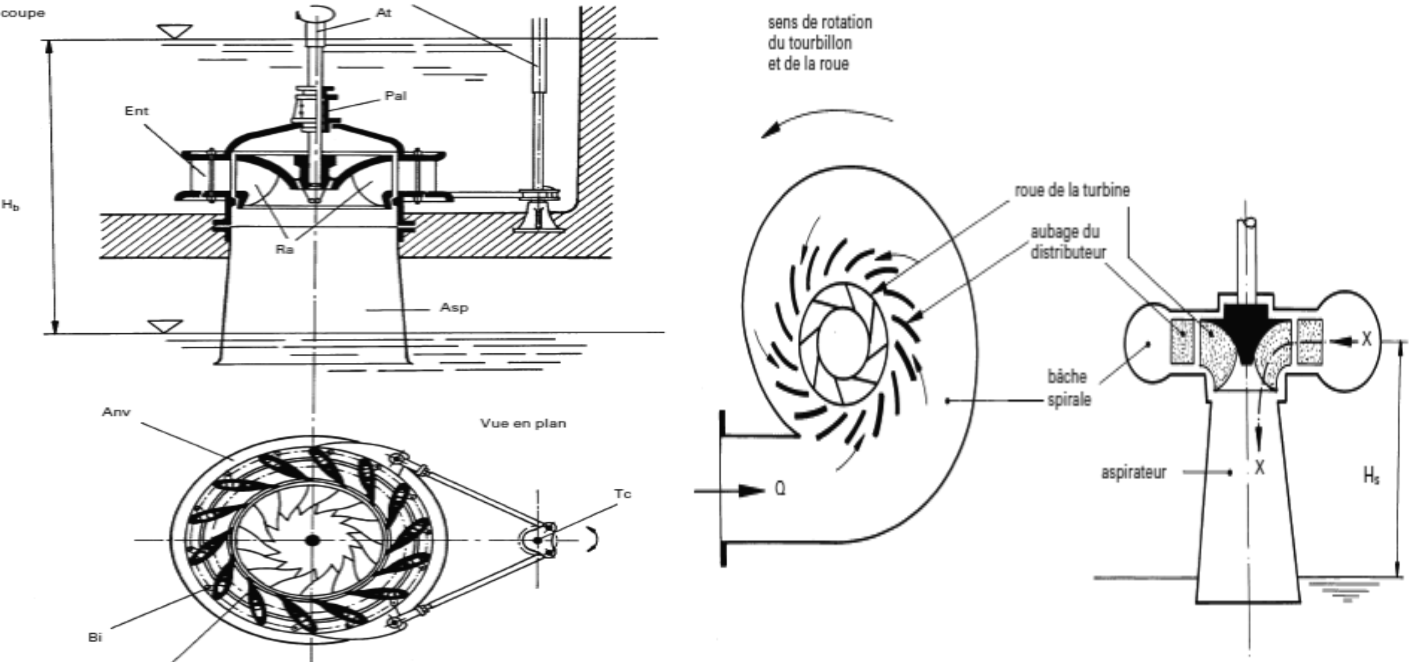
\includegraphics[scale=0.4]{ch4/8}
\captionof{figure}{}
\end{center}
The Francis turbine has fixed geometry rotor blades, but movable vanes (changing pitch angle) on the distributor. The flow enters in a spiral casing that will evenly distribute water using the vanes. Again, we have horizontal and vertical configurations. The first is used for low heads and low power while the other for high heads and powers because of high axial thrust and large bearings are required.\\

It is designed to work on medium heads (3 - 350 m) and medium flows (0.4 to 30 $m^3/s$) and can develop important power. It has a rpm of 100 to 1000 and can overspeed up to 230\%. On the other hand, the design and engineering are very complex requiring the knowledge of group dynamic and ensuring high reliability. 

\subsection{Propeller and Kaplan turbines}
\begin{center}
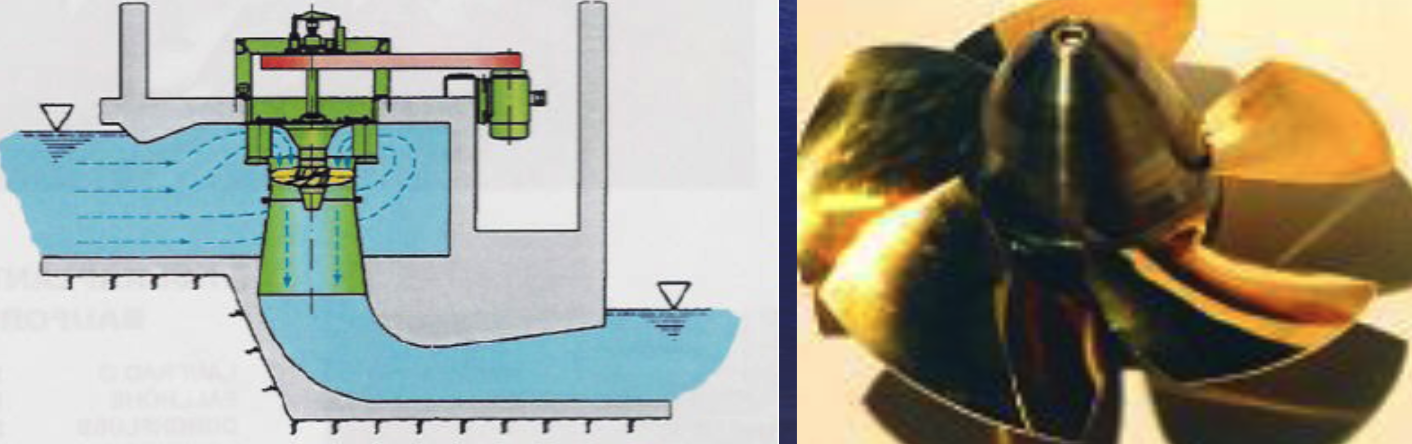
\includegraphics[scale=0.4]{ch4/9}
\captionof{figure}{}
\end{center}

These are wheels similar to boat propellers with fixed blades (propeller) or movable (Kaplan). The flow properties (spiral, ...) are similar to the Francis turbine but in Kaplan the flow is purely axial as represented on the figure. The flow is redirected towards the center of the propeller by the fixed or adjustable distributor. When leaving, we have a divergent aspirator to limit turbulences. \\

These are designed to work on small to medium heads (3-50 m) and high flow rate (0 - 5 $m^3/s$). They are classified according to their provision: bulb turbine, siphon turbine, turbine in S (upstream and downstream), submerged turbine monoblock. 

\subsection{Inverted pumps}
These are pumps with inverted flow direction and inverted shaft rotation. Operation similar to the Francis but with lower specific speed and fixed distributor vanes. It is cheap, easy to install and compact. Used for low heads, but has many disadvantages: 

\begin{itemize}
\item[•] constant flow rate,
\item[•] if sudden discharge, high risk of water hammer in the pipe,
\item[•] need a flywheel because of fast speed transition,
\item[•] additional engineering to make it operational in inverse mode, 
\item[•] the reversing of the rotation direction takes time,
\item[•] lower efficiency than Francis turbine operating in the same conditions. 
\end{itemize}

\begin{center}
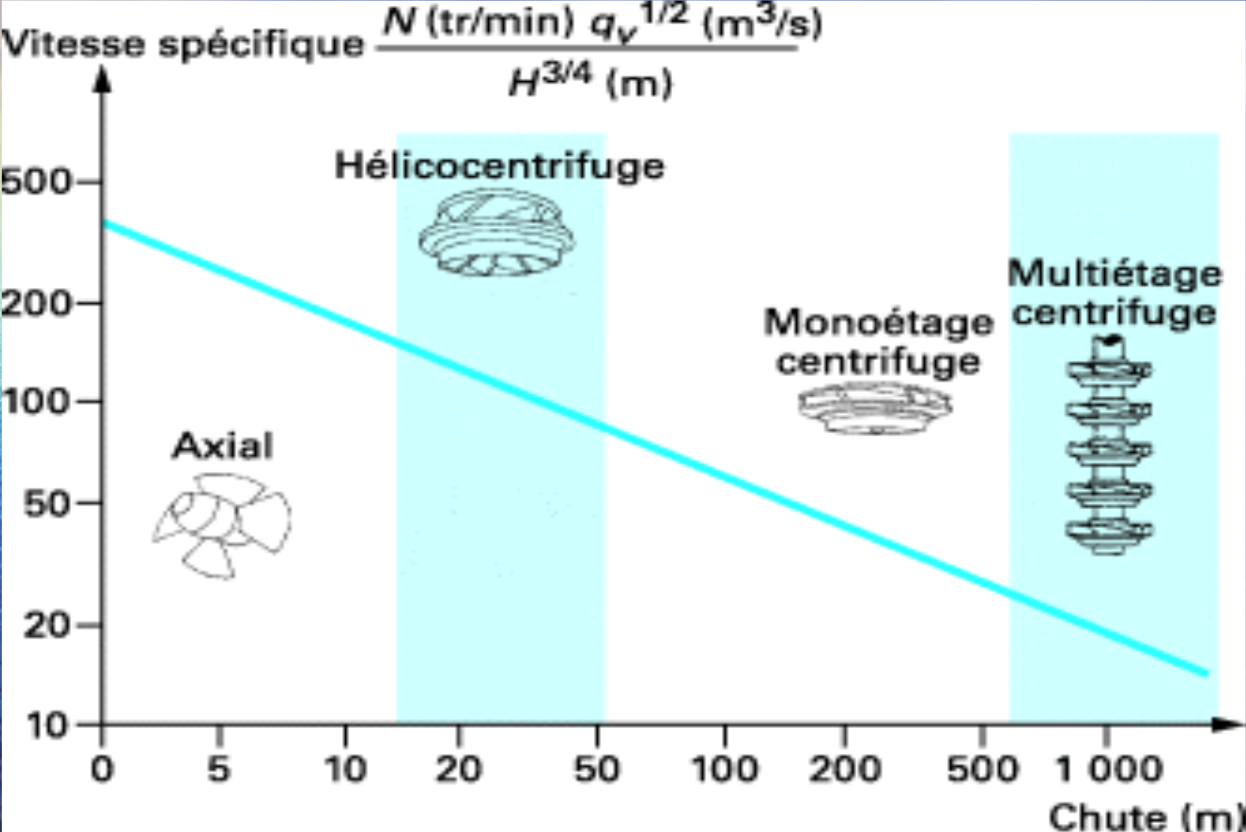
\includegraphics[scale=0.3]{ch4/10}
\captionof{figure}{}
\end{center}

\subsection{Archimedes turbines}
\wrapfig{7}{l}{7}{0.3}{ch4/11}
Hydrodynamic screw generates energy by letting the water run into the screw down (it rotates). This is in fact also an inverted pump. It is not submerged and supported by 2 bearings (one of them is thus in the water and is a friction problem). It is used for low head and small or medium flow rates. \ \\\\\\

\wrapfig{7}{r}{6}{0.5}{ch4/12}
Advantages and disadvantages:  
\begin{itemize}
\item[+] Compared to other turbines of the same magnitude, the screw has a similar or higher efficiency. 
\item[+] Wide range of good efficiency,
\item[+] fish-friendly, no fine grids, 
\item[+] robust, simple, not expensive and low maintenance.
\item[-] low power, low speed requires multiplier so losses, sealing and lubrication of bottom bearing. 
\end{itemize}

\section{Performance curves and operating conditions}
\begin{center}
\begin{minipage}{0.3\textwidth}
\begin{center}
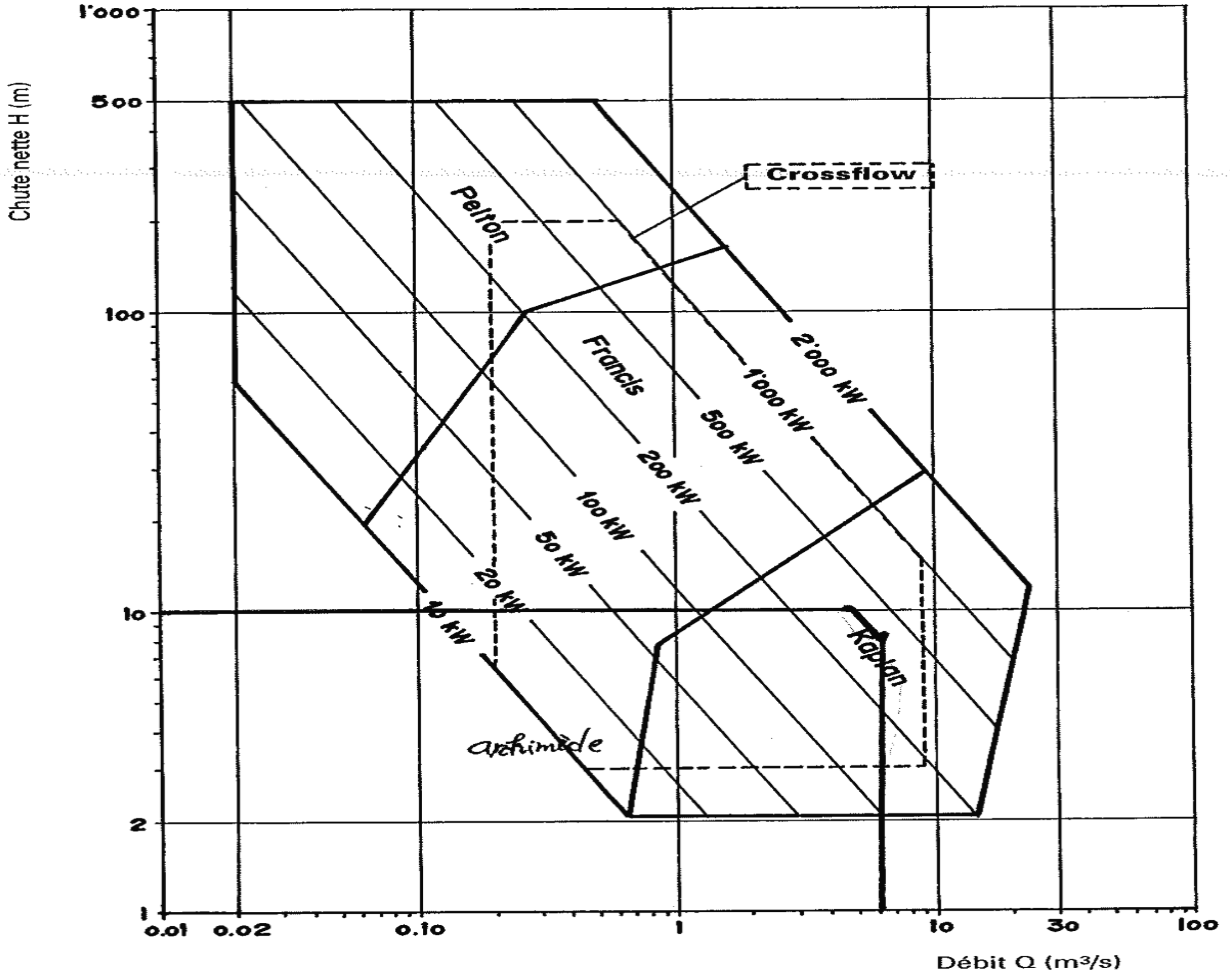
\includegraphics[scale=0.2]{ch4/13}
\end{center}
\captionof{figure}{}
\end{minipage}
\quad
\begin{minipage}{0.3\textwidth}
\begin{center}
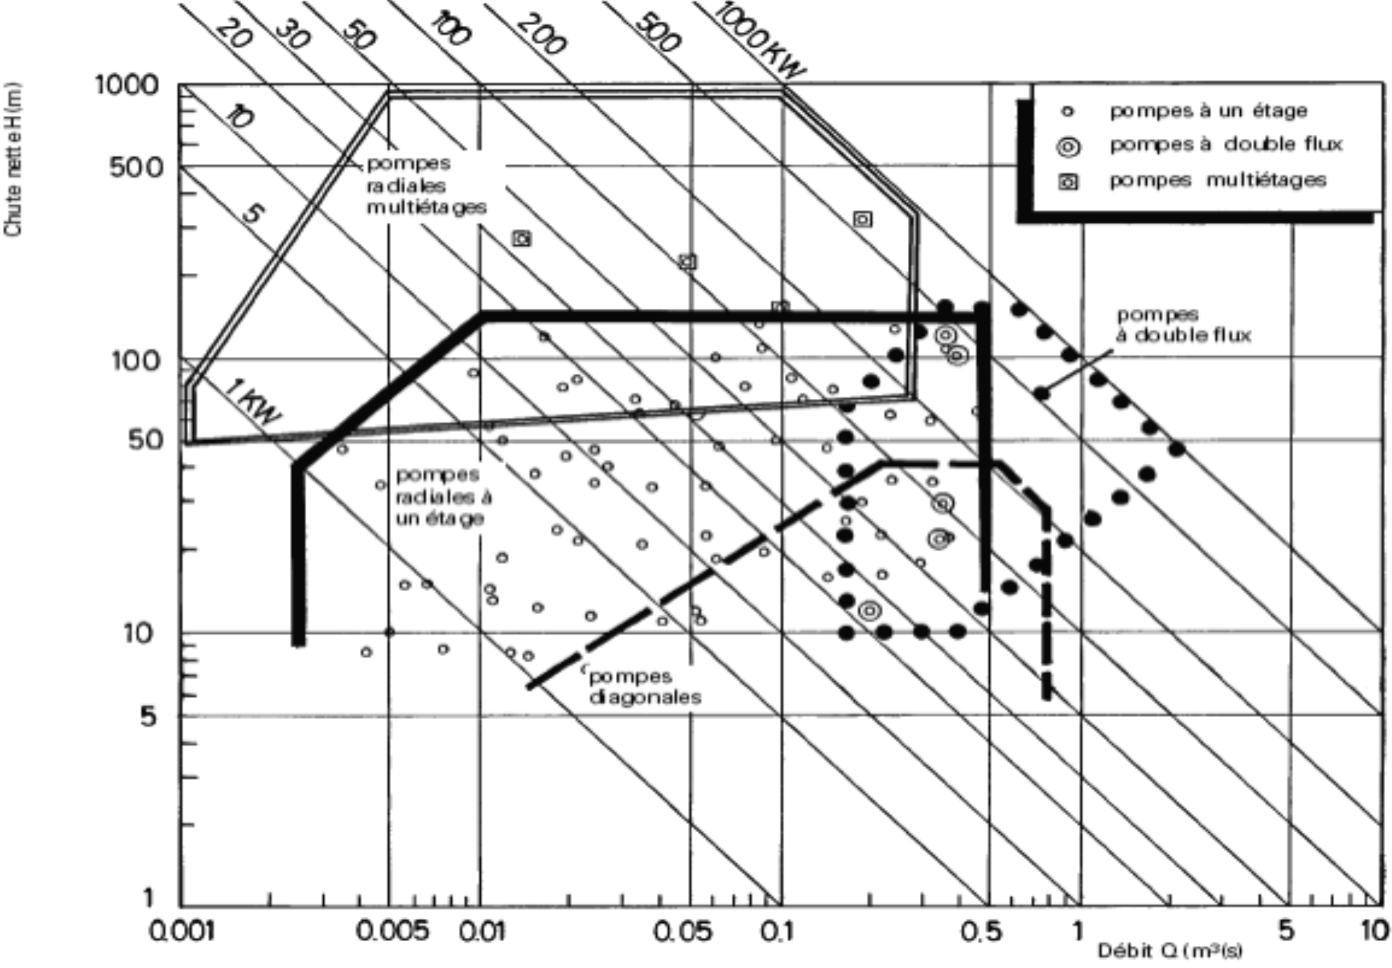
\includegraphics[scale=0.2]{ch4/14}
\end{center}
\captionof{figure}{}
\end{minipage}
\quad
\begin{minipage}{0.3\textwidth}
\begin{center}
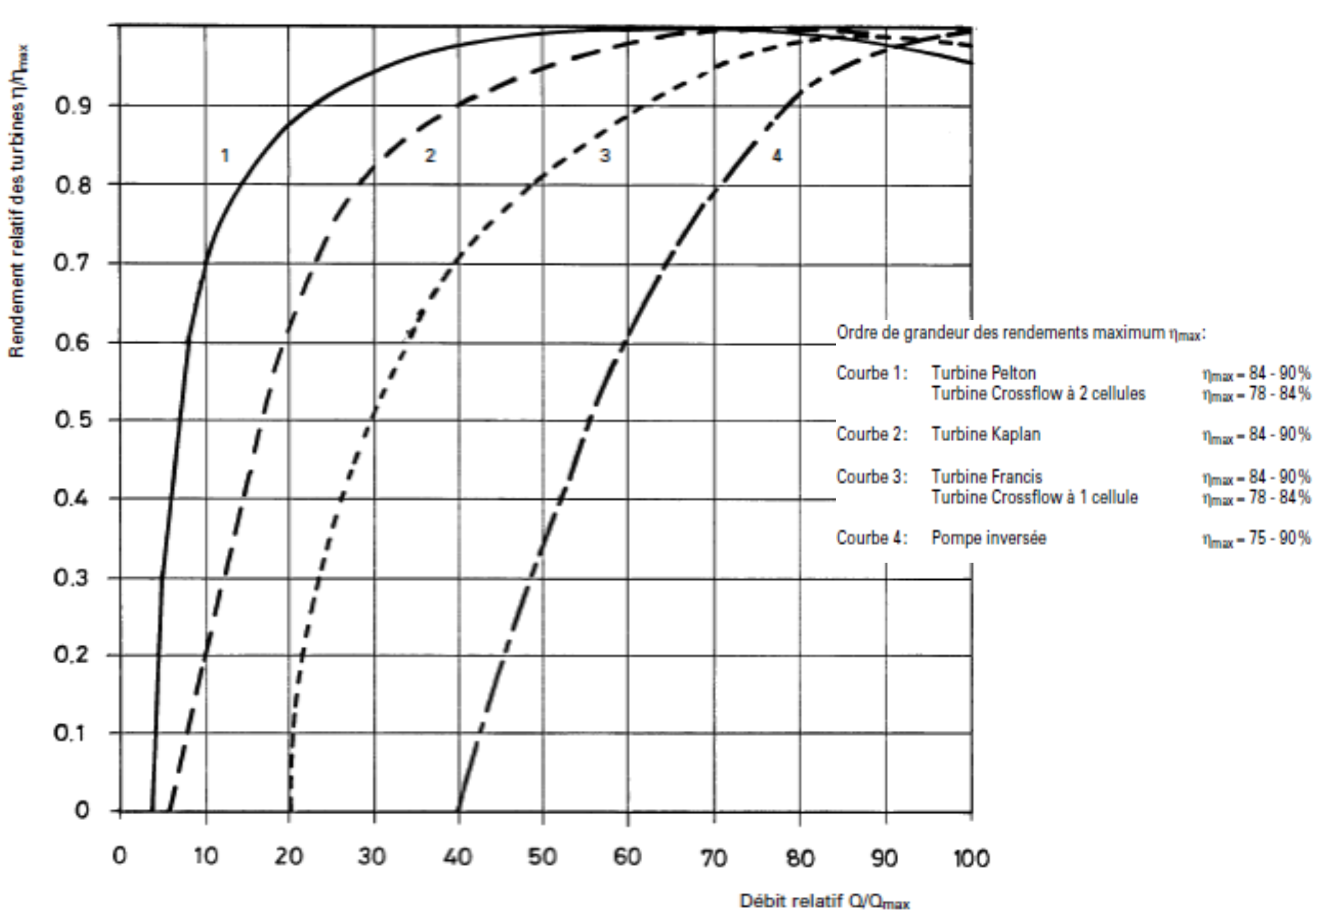
\includegraphics[scale=0.22]{ch4/15}
\end{center}
\captionof{figure}{}
\end{minipage}
\end{center}


\wrapfig{12}{l}{6}{0.3}{ch4/16}
The two first figures represent the power curves in function of the head and the flow rate. The third figure shows the efficiency. All what we have discussed previously are summarized here. 
\ \\

The grid has a fixed frequency (50 Hz in Belgium), and thus the maximum rotation speed is limited in function of the number of poles of the generator. It is possible to select the turbine in function of the rotation speed, knowing the flow rate (at left of the graph) and the head (right) as shown on the figure. 
\ \\

\subsection{Implementation of a hydroturbine}
\wrapfig{10}{l}{7}{0.3}{ch4/17}
We said that the pressure at the entrance of the pump (minimum section) must be higher than the saturation pressure otherwise we have cavitation. We put the pump lower than the upstream water level. Here we introduce the suction head, distance between the central shaft of the turbine and the level of water in the lower reservoir. This suction head is important because it is lost energy in fact. Depending on the type of turbine, the suction head will be different, this is summarized on the figure. This implies that for low head turbines, the location on the circuit may be different from type to type. 

\subsection{Turbine generator group layout}
There are 3 main possibilities: turbine on the shaft of the generator, both with different shafts but directly coupled and the one with the transition of a speed multiplier (belt, gear). 

\section{Summary}
\minifig{ch4/18}{ch4/19}{0.3}{0.6}{0.45}{0.45}

\minifig{ch4/20}{ch4/21}{0.5}{0.3}{0.45}{0.45}